\textbf{\hypertarget{P6}{[\,Suggested Time: 40 mins \textbar \, Total Marks: 20 \textbar \, Challenging\,]}}\\\\
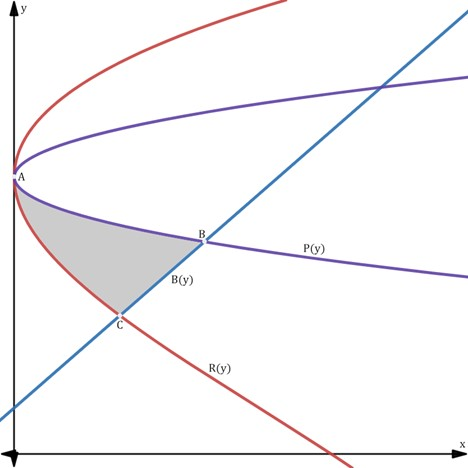
\includegraphics[scale=1]{Question 6 - Graph.jpg}\\
\textit{
    \textbf{Answers by Accurate drawings or graphical methods are not accepted.}\\
    The graphs are plotting y against x. Point A is a common stationary point of\\
    R(y) and P(y). B(y) passes through the points \(D(10 , 2)\) and \(E(1 , \frac{1}{2})\).\\
    \(P(y) = 33(y - 2)^2\) , \(B(y) = R''(y)\)\\
    Degree of polynomial R(y) is 3.
}

    \newpage

\textit{Find the shaded area.\\*
        \textbf{Leave your answers in exact values,} in the form \(a + b\sqrt{339}\) , where $a, b\in\mathbb{Q}$
} \qnmark{20}

%%%%%%%%%%%%%%%%%%
%%%%%Solution%%%%%
%%%%%%%%%%%%%%%%%%

%\newpage \ \newpage \ \newpage \ \newpage

%\begin{comment}

%%%%%Showing that B(y) is linear%%%%%
\begin{gather*}
    Degree \; of \; R(y) \; is \; 3 \implies Degree \; of \; B(y) \; is \; 1, \; therefore \; B(y) \; is \; a \; linear \; function
\end{gather*}

%%%%%Finding B(y)%%%%%
\textit{Finding the Equation of B(y)}
\begin{align*}
    \displaystyle   y-2 &= \frac{1}{6}(x-10) \\
    \displaystyle 6y-12 &= x-10 \\
    \displaystyle     x &= 6y-2 \\
    \displaystyle \therefore B(y) &= 6y-2 \onemark \\
\end{align*}

%%%%%Finding R(y) & Point A%%%%%
\textit{Finding the coordinates of point A}
\begin{equation*}
    \displaystyle P'(y) = 66(y-2)
\end{equation*}
\textit{When P(y) = 0}
\begin{align*}
    66(y-2) &= 0 \\
    \therefore y &= 2 \onemark
\end{align*}
\textit{Sub y = 2 into P(y)}
\begin{align*}
    \therefore x &= 33(2-2)^{2}\\
                &= 0 \\
    \implies  A &= (0 , 2) \onemark
\end{align*}

\textit{Finding the equation of R(y)}\\
\textit{Since B(y) = R''(y)}
\begin{align*} %% Finding R'(y)
    \displaystyle R'(y) &= \int{B(y)} \; dy\\
    \displaystyle       &= 3y^{2}-2y+c_{1} , where \; c_{1}\in\mathbb{R} \onemark\\
\end{align*}
\textit{Point A is a stationary point of R(y)\(\implies R'(2) = 0\)}
\begin{align*} %% Finding c_1
    3(2)^{2}-2(2)+c_{1} &= 0 \\
                  c_{1} &= -8 \onemark \\
    \therefore    R'(y) &= 3y^{2}-2y-8
\end{align*}

\newpage

\begin{align*} %% Integrating R'(y)
    R(y) &= \int{R'(y)} \; dy \\
         &= y^{3}+y^{2}-8y+c_{2} , where \; c_{2}\in\mathbb{R} \onemark
\end{align*}
\textit{When x = 0, y = 2,}
\begin{align*}
                  R(2) &= 0 \\
    2^{3}-2{2}-8+c_{2} &= 0 \\
    \therefore  c_{2} &= 12 \onemark \\
    \implies R(y) &= y^{3}-y^{2}-8+12 \\
\end{align*}

%%%%%Finding Points B & C%%%%%
\textit{Given that Point C is an intercept of R(y) and B(y)}
\begin{align*} %% Rewriting R(y) =B(y)
    \displaystyle               R(y) &= B(y) \\
    \displaystyle  y^{3}-y^{2}-8y+12 &= 6y-2 \\
    \displaystyle y^{3}-y^{2}-14y+14 &= 0 \onemark
\end{align*}
\begin{align*} %% Solving the equation
    \displaystyle Let \; f(x) &= y^{3}-y^{2}-14y+14 \\
    \displaystyle f(1) &= 0
\end{align*}
\begin{gather*}
    \displaystyle \therefore (y-1) \; is \; a \; factor \; of \; f(x) \onemark
\end{gather*}
\begin{align*} %% Finding the y-coordinate of C
     f(x) &= (y-1)(y^{2}-14) \\
          &= 0 \\
    \\
    y^{2} &= 14 \\
        y &= \pm\sqrt{14} \\
    \therefore y &= 1 \; or \pm\sqrt{14}
\end{align*}
\begin{gather*}
    Rej. \; y = \pm\sqrt{14} \\
        \implies y = 1 \onemark \\
\end{gather*}
\begin{align*} %% Finding the x-coordinate of C
    Sub. \; y &= 1 \; into \; B(y), \\
    B(1) &= 6(1)-2 \\
         &= 4 \\
    \therefore C &= (4,1) \onemark
\end{align*}

\newpage

%%%%%Finding Point B%%%%%
\textit{Given that Point B is an intercept of P(y) and B(y)}
\begin{align*} %% Rewriting the Equation
    \displaystyle 6y-2 &= 33(y-2)^{2} \onemark \\
    \displaystyle      &= 33y^{2}-132y+132
\end{align*}
\begin{equation*}
    \displaystyle 33y^{2}-138y+134 = 0 \\
\end{equation*}
\begin{align*} %% Finding the values of y
    y &= \frac{138\pm\sqrt{(-138)^{2}-4(33)(134)}}{2(33)} \\
      &= \frac{138\pm\sqrt{1356}}{2(33)} \\
      &= \frac{69\pm\sqrt{339}}{33} \onemark
\end{align*}
\textit{Reject $\displaystyle y = \frac{69+\sqrt{339}}{33}$, $\displaystyle \therefore y = \frac{69-\sqrt{339}}{33}$} \\
\\\\
\textit{Sub $\displaystyle y = \frac{69-\sqrt{339}}{33}$ into B(y)}
\begin{align*} %% Finding Point B
    \displaystyle B\left(\frac{69-\sqrt{339}}{33}\right) &= 6\left(\frac{69-\sqrt{399}}{33}\right)-2 \\
    \displaystyle                                        &= \frac{2\left(69-\sqrt{339}\right)-22}{11} \\
    \displaystyle                                        &= \frac{116-2\sqrt{339}}{11}
\end{align*}
\begin{equation*}
    \displaystyle \therefore B = \left(\frac{116-2\sqrt{339}}{11},\frac{69-\sqrt{339}}{33}\right) \onemark \\
\end{equation*}

\newpage

%%%%%Finding the shaded area%%%%%
\textit{Let S be the shaded area and \(\displaystyle \alpha = \frac{69-\sqrt{339}}{33}\)}
\begin{align*}
    \displaystyle S &= \int_{\alpha}^{2} P(y) \, dy + \frac{1}{2}\left(\frac{69-\sqrt{339}}{33}-1\right)\left(\frac{116-2\sqrt{339}}{11}+4\right) - \int_{1}^{2} R(y) \, dy \\
    \displaystyle   &= \int_{\alpha}^{2} 33(y-2)^{2} \, dy + \frac{1}{2}\left(\frac{69-\sqrt{339}}{33}-1\right)\left(\frac{116-2\sqrt{339}}{11}+4\right) - \int_{1}^{2} y^{3}-y^{2}-8y+12 \, dy \onemark \\
    \displaystyle   &= \left[11(y-2)^3\right]_{a}^{2} + \frac{1}{2}\left(\frac{36-\sqrt{339}}{33}\right)\left(\frac{160-2\sqrt{339}}{11}+4\right) - \left[\frac{y^{4}}{4}-\frac{y^{3}}{3}-4y^{2}+12y\right]_{1}^{2} \onemark \\
    \displaystyle   &= -11\left(\frac{69-\sqrt{339}}{33}-2\right)^{3} + \frac{\left(36-\sqrt{339}\right)\left(160-2\sqrt{339}\right)}{726} \\
    \displaystyle   &  -\left(\frac{2^{4}}{4}-\frac{2^{3}}{3}-4(2)^{2}+12(2)-\left(\frac{1}{4}-\frac{1}{3}-4+12\right)\right) \onemark \\
    \displaystyle   &= -11\left(\frac{3-\sqrt{339}}{33}\right)^{3}+\frac{6438-232\sqrt{339}}{726}-\frac{17}{12} \\
    \displaystyle   &= \frac{-44\left(3078-366\sqrt{339}\right)+99\left(12029-464\sqrt{339}\right)}{143748} \\
    \displaystyle   &= \frac{1055439-62040\sqrt{339}}{143748}  \\
    \displaystyle   &= \frac{10661}{1452}-\frac{470}{1089}\sqrt{339} \\
    \\
    \displaystyle   &  \therefore the \; shaded \; area \; is \left(\frac{10661}{1452}-\frac{470}{1089}\sqrt{339}\right) \, u^{2} \onemark
\end{align*}
%\end{comment}